\documentclass[../phys-f308.tex]{subfiles}

\begin{document}
    \part{Intermolecular forces}
    \begin{abstract}
        In the study of matter, one defines several different states. In this course, we will focus on the study of the properties of condensed matter. Crystals and liquids are examples of such condensed matter - the interaction between molecules of the latter is of the order of $E_{int}>> k_BT$ whereas the former preents an interaction energy $E_{int}\geq k_BT$ which can be put in contrast to a gas' $E_{int}<< k_BT$. Let us note that thermal energy is much larger than the interactions between particules in the gaseous states. 
    \end{abstract}

    \section{Microscopic interaction potential}

    Let us consider the interaction between two different molecules. The total energy in the system can be written as
    \begin{equation}
        E_{tot}(r) = E_A+E_B+w(r)
    \end{equation}
    where $r$ is the distance between the molecules $A$ and $B$ and $w(r)$ is the \emph{potential of interaction}, defined as
    \begin{align}
        w(r) &= E_{tot}(r) - E_{tot}(\infty)\\
        w(r) &= -\int_r^{\infty}F(r)dr \quad \Leftrightarrow \quad F(r) = -\frac{dw}{dr}\label{eq: F dw/dr}
    \end{align}
    Beware to the minus sign between the two: the interaction is \emph{attractive} when the potential is negative, and \emph{repulsive} when the potential   

    \section{L1 : Molecular interactions via electrostatic potentials}

    We will perform a review of the electrostatic potential interaction, with an increasing level of complexity. In particular, we will consider the interaction between...
    \begin{itemize}
        \item Two single point charges (approximation for two ions), dipole moments (approximation for two molecules)
        \item A single point charge and a non-rotating dipole moment
        \item Two non rotating dipole moments
        \item A single point charge and a rotating dipole moment
        \item Two rotating dipole moments
    \end{itemize}

    \subsection{Electrostatic interaction between two point charges}
    Let us consider two single points charges $Q_1$ and $Q_2$ separated by a distance $r$. As a reminder, let us note that the electric field of a charge $Q$ at a distance $r$ is given by $E = \frac{Q}{4\pi\epsilon_r\epsilon_0 r^2}$. Therefore, the electric force of charge $Q_1$ on charge $Q_2$ is given by $F=E_1Q_2 = \frac{Q_1Q_2}{4\pi\epsilon_r\epsilon_0 r^2} = \frac{z_1z_2 e^2}{4\pi\epsilon_r\epsilon_0 r^2}$ by introducing the valence numbers $z_i$. We deduce the macroscopic electrostatic potential
    \begin{equation}
        w(r) = -\frac{z_1z_2e^2}{4\pi\epsilon_r\epsilon_0 r}
    \end{equation} 

    \paragraph{Electrostatic interaction: application to $NaCl$}

    In a vaccum, one finds that $w_{NaCl} = -8.4\ti 10^{-19}J$. However, at room temperature one has that $U_T = k_BT \approx 1.38\ti 10^{-23} J/K \cdot 291 J = 4\ti 10^{-21}J$. Given that \color{red}$w_{NaCl}>200 k_BT$\footnote{Why do we ignore the negative sign?}\color{black}, NaCl is stable at room temperature in a vaccum. However, put it in a medium with high dielectric constant such as water and $w_{NaCl}^{H_2O}(r) \approx 2.5 k_BT$.

    \subsubsection{Dipole moments}

    Asymetric molecules bounded by covalent bounds often contains dipole moments. One defines the units of $Debye$ for this purpose: take two charges $e$ and $-e$ separated by a distance of one $Angstrum$:
    \begin{equation*}
        \mu = 4.8 D
    \end{equation*}

    \paragraph{Dipole moment of water}

    \begin{example}
        The molecule of water can be seen as two $OH$ molecules separated by an angle of $104.5°$. Given that $\mu_{OH} = 1.51 D$, we deduce that the dipole moment of water is given by 
        \begin{equation}
            \mu_{H_2O} = 2\cos\left(\frac{H\hat{O}H}{2}\right)\mu_{HO} = 1.85D
        \end{equation}
    \end{example}

    \subsubsection{Ion-dipole interaction}

    Instead of looking a two single point charges and a dipole seperately, let us put them together and see what happens as shown in figure \ref{fig: ion-dipole interaction}. The resulting macroscopic electrostatic potential is
    \begin{equation}
        w(r) = -\frac{qQ}{4\pi\epsilon_0r_A}+\frac{qQ}{4\pi\epsilon_0r_B} = \frac{qQ}{4\pi\epsilon_0}\left(\frac{1}{r_B}-\frac{1}{r_A}\right)\label{eq: ion-dipole interaction 1}
    \end{equation}

    Let us note that $r_A \approx r-\frac{l}{2}\cos\theta$ whereas $r_B\approx r+\frac{l}{2}\cos\theta$. Applying the approximation $\frac{r_A-r_B}{r_Ar_B}\approx -\frac{l\cos\theta}{r^2}$, one finds that  \eqref{eq: ion-dipole interaction 1} can be rewritten as
    
    \begin{equation}
        w(r) \approx -\frac{qQ}{4\pi\epsilon_0}\frac{l\cos\theta}{r^2} = -\mu\frac{Q\cos\theta}{4\pi\epsilon_0r^2} \quad w(r) = -\mu E(r)\cos\theta
    \end{equation}

    The potential is either attractive or repulsive, depending on the orientation of the molecule.

    \begin{figure}[h!]
        \centering
        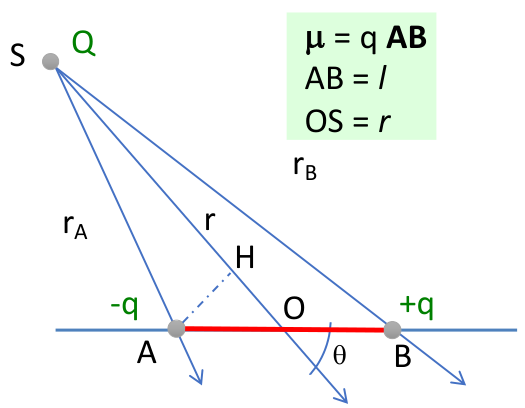
\includegraphics[width=50mm]{partA/Pictures/DipoleIon.png}
        \caption{Ion-dipole interaction}
        \label{fig: ion-dipole interaction}
    \end{figure}

    \subsubsection{Ion-ion interaction}

    \part{Phase transitions I : Thermodynamics}

    Test

\end{document}